% LCS: voodoo for arXiv scripts, must appear in the first 4 lines
\pdfoutput=1
\documentclass[aps,prd,twocolumn,superscriptaddress,preprintnumbers,floatfix,nofootinbib]{revtex4-2}
%\documentclass[aps,prl,preprint,superscriptaddress]{revtex4-1}
%\documentclass[aps,prl,reprint,groupedaddress]{revtex4-1}

\usepackage{graphicx}
\usepackage{amsmath, amssymb, mathrsfs}
\usepackage{color}
\usepackage{bm}
% LCS: Proper input/output encoding
\usepackage[T1]{fontenc}
\usepackage[utf8]{inputenc}
\usepackage{microtype}
\usepackage[normalem]{ulem}
\usepackage[dvipsnames]{xcolor}
\usepackage[colorlinks,urlcolor=NavyBlue,citecolor=NavyBlue,linkcolor=NavyBlue,pdfusetitle]{hyperref}
\usepackage[all]{hypcap}
\usepackage{orcidlink}

\usepackage{lipsum}

\newcommand{\NR}{\text{NR}}

% LCS: Directories for figures. This makes life easier for moving
% figures around.
\graphicspath{{figs/}}

%% Try to control orphans, widows, and extra whitespace
%\widowpenalty=10000
%\clubpenalty=10000
%\raggedbottom
%\interfootnotelinepenalty=3000

\newcommand{\Note}[1]{\textcolor{red}{\textbf{[#1]}}}
\newcommand{\lcs}[1]{\textcolor{WildStrawberry}{#1}}

\begin{document}


%Title of paper
\title{Notes on XXX}

\author{Leo C.\ Stein\,\orcidlink{0000-0001-7559-9597}}
\email[]{lcstein@olemiss.edu}
%\thanks{}
%\altaffiliation{}
\affiliation{Department of Physics and Astronomy,
    University of Mississippi, University, MS 38677, USA}

% Because hyperref only gets the *last* author, we need to be explicit.
%\hypersetup{pdfauthor={Stein}}

\date{\today}

\begin{abstract}
  Here is our abstract.
  Some well known problem.
  Currently limitation of the field.
  Here we solve the problem.
  This leads to result of ABC.
\end{abstract}

%\maketitle must follow title, authors, abstract
\maketitle

%\tableofcontents

\section{Introduction}
\label{sec:introduction}

As is by now well known, black hole entropy is a Noether
charge~\cite{Wald:1993nt, Noether:1918zz}.
\lipsum[1]

\section{Results}
\label{sec:results}

We used matched asymptotic expansions~\cite{bender1999advanced}.
%
\begin{figure}[t]
  \begin{center}
    %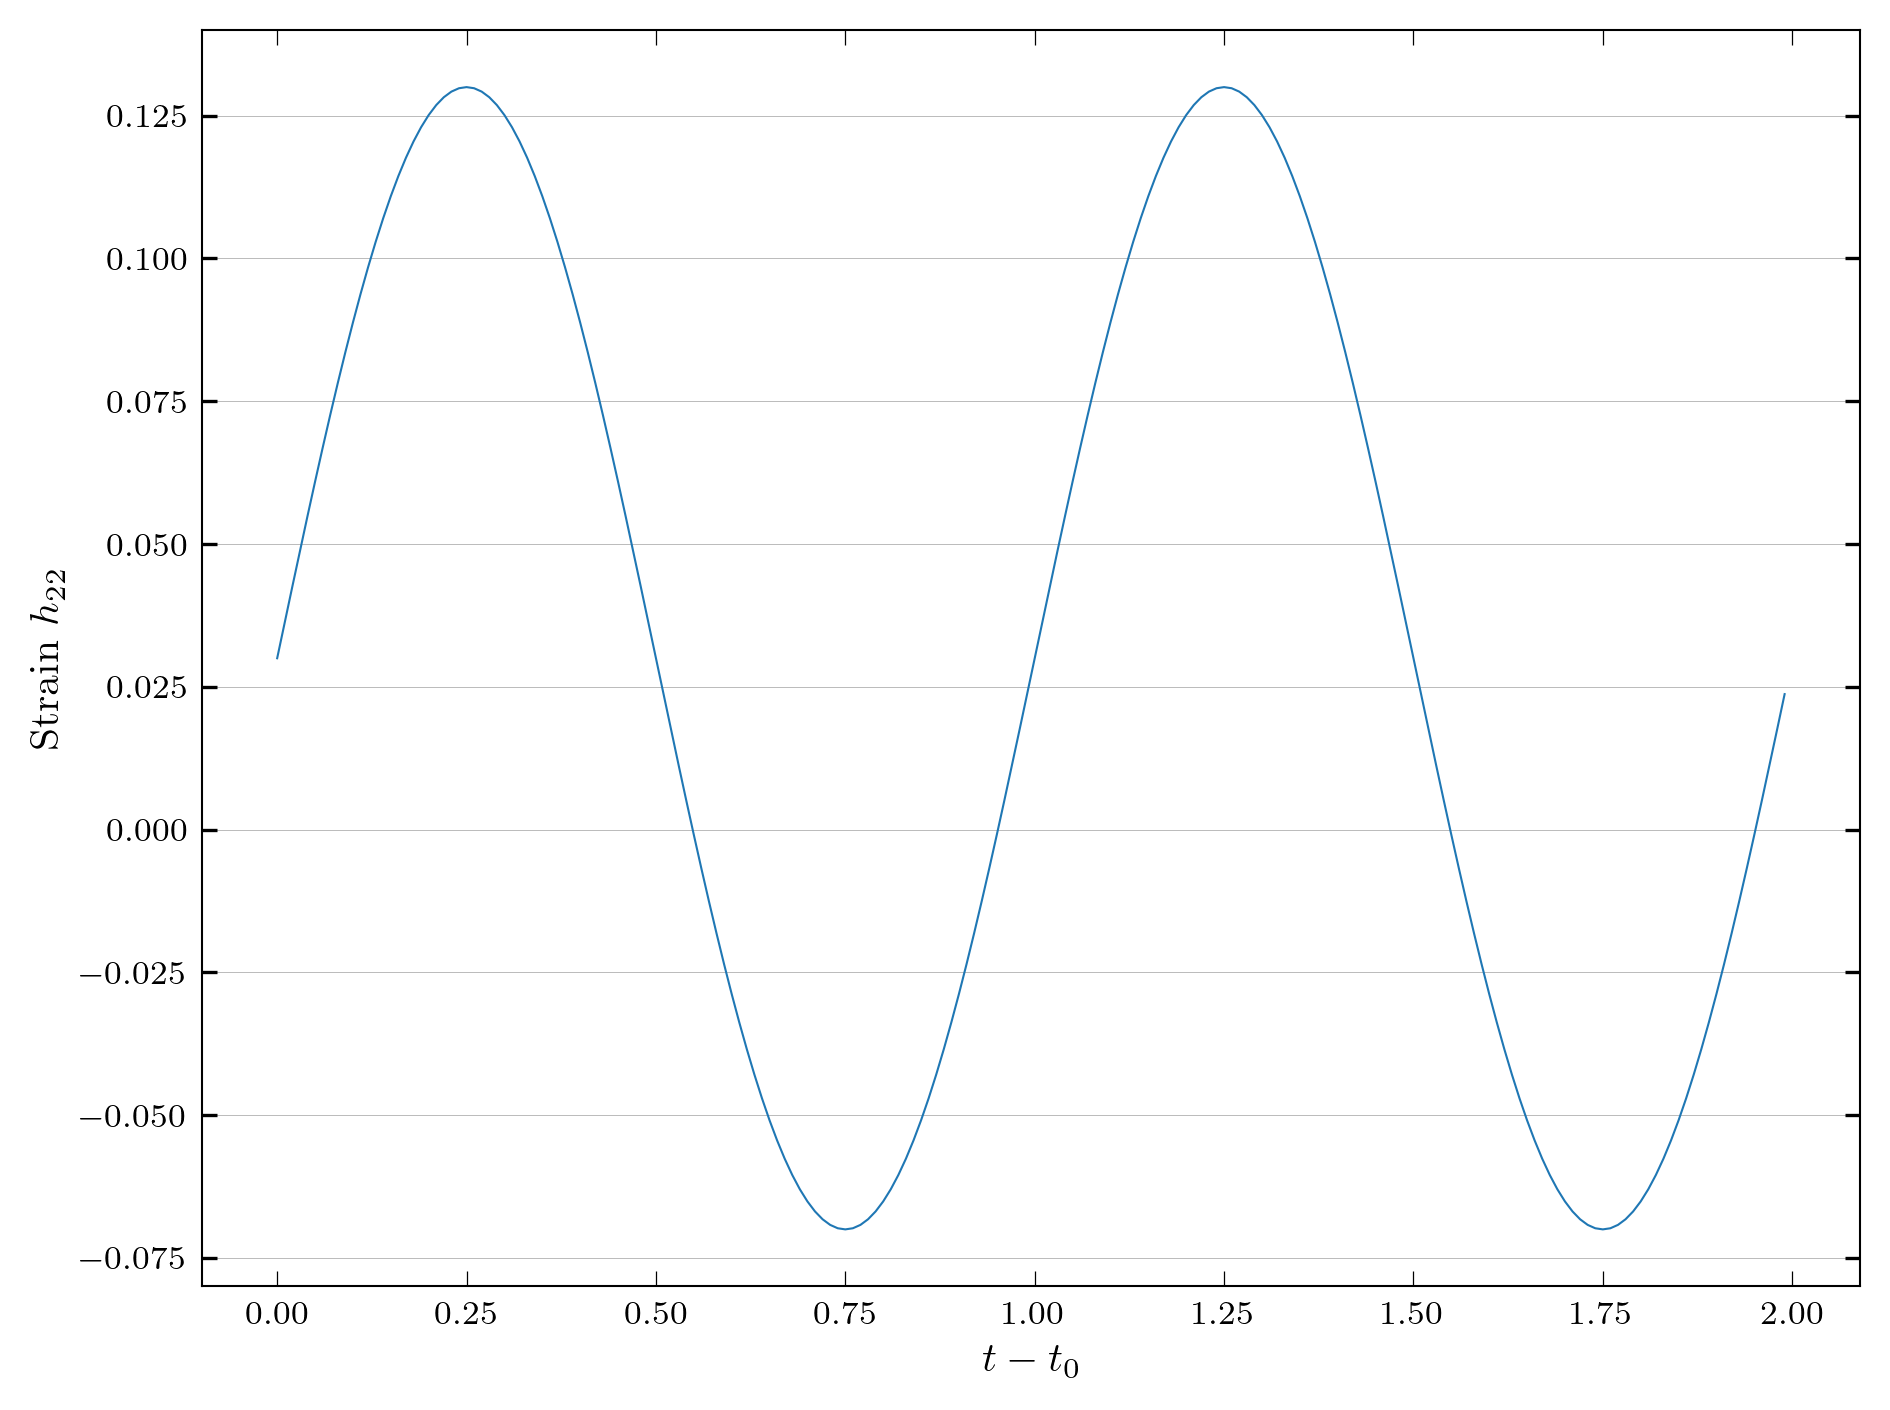
\includegraphics[width=\columnwidth]{use_style}
    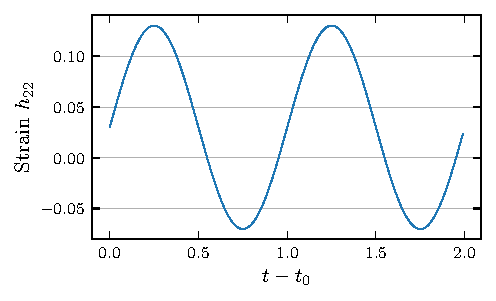
\includegraphics[width=\columnwidth]{specified_size}
  \end{center}
  \vspace{-\baselineskip}
  \caption{%
    Isn't this figure so lovely? We all just love making figures in
    \texttt{matplotlib}.}
  \label{fig:lovely}
  \vspace{-\baselineskip}
\end{figure}
%
\lipsum[2-4]

\section{Discussion and conclusions}
\label{sec:disc-concl}

In this article, we solved the previously open problem of XYZ.
\lipsum[5]

\subsection{Future work}
\label{sec:future-work}

Our method can be adapted for generalizations.

\acknowledgments
%
The authors would like to thank
%
TODO
%
for useful discussions.

% \appendix
% Put messy things here

\bibliographystyle{JHEP}
\bibliography{notes-biblio}

\end{document}

% Local Variables:
% mode: latex
% End:
